\documentclass[12pt]{article}  % [12pt] option for the benefit of aging markers

% amssymb package contains more mathematical symbols
\usepackage{amssymb,amsthm}
\usepackage{amsmath}

% graphicx package enables you to paste in graphics
\usepackage{graphicx}
\usepackage{auto-pst-pdf}
\usepackage{subfig}

% embed source inside latex
\usepackage[procnames]{listings}
\usepackage{color}

% ALGORITHM
\usepackage{algorithm}
\usepackage{algpseudocode}
\usepackage{hyperref}
\usepackage{booktabs}
\usepackage{enumitem}

%%%%%%%%%%%%%%%%%%%%%%%%%%%%%%%%%
%
%    Page size commands.  Don't worry about these
%
\setlength{\textheight}{220mm}
\setlength{\topmargin}{-10mm}
\setlength{\textwidth}{150mm}
\setlength{\oddsidemargin}{0mm}

%%%%%%%%%%%%%%%%%%%%%%%%%%%%%%%%%%%%%%%%%%%%%%%%%%%%%%%%%%%%%%%
%
%    Definitions of environments for theorems etc.
%
\newtheorem{theorem}{Theorem}[section]          % Theorems numbered within sections - eg Theorem 2.1 in Section 2.
\newtheorem{corollary}[theorem]{Corollary}      % Corollaries etc. will be counted as Theorems for numbering
\newtheorem{lemma}[theorem]{Lemma}              % eg Lemma 3.1, ... Theorem 3.2, ... Corollary 3.3.
\newtheorem{proposition}[theorem]{Proposition}
\newtheorem{conjecture}[theorem]{Conjecture}

\theoremstyle{definition}
\newtheorem{definition}[theorem]{Definition}

\theoremstyle{remark}
\newtheorem{remark}[theorem]{Remark}
\newtheorem{example}[theorem]{Example} 

%%%%%%%%%%%%%%%%%%%%%%%%%%%%%%%%%%%%%%%%%%%%%%%
%
%        Preamble material specific to your essay
%
\title{Simulating M/M/2/2+5 Queueing System}
\author{Jiaqi Yan, Ping Liu\\
CS555 Project\\
supervised by
Edward Chlebus}

\begin{document}
\maketitle

% \newpage                     % optional page break
\begin{abstract}
In this project, we simulate and analyze the \textbf{M/M/2/2+5 queueing system}. 
To generate packet arriving time and service time, we use Python's built-in \textit{random} module, which is validated carefully.
Then we apply the \textbf{Welch graphical procedure} to eliminate the warm-up period in the simulation.
With the stationary region, we then analyze the system's properties such as blocking probability and mean number of packet in the system.
The \textbf{90\% confidence intervals} for these properties are also given.
\end{abstract}

% optional page break
\newpage
\tableofcontents

% optional page break
\newpage
\section{Discrete Event Simulation}\label{sec:des}
We designed and implemented our own simple simulator for M/M/2/2+5 queueing system.
The simulation workflow is shown in Algorithm \ref{alg:simulator}.
The whole process is embedded inside a while loop.

The while loop will keep consume event in the $event\_list$ until we handled all the packets.
Whenever there is unseen packets, we create an arrival event and insert it to the list.
This list thus should be maintained in order with respect to events' time stamp, which is determined as soon as we create a \texttt{event} object.
Also based on this time stamp, we will pop up the next event we should handle from the list according to the event type, either $arrival$ or $departure$.

If the type is $departure$, we first check number of arrived but waiting packets in the system.
When no packets need to be served at this moment, set the server this packet is leaving from to $idle$;
otherwise, just decrease this $waiting$ counter.
Anyway, we just served a packet.
This means the counter for served packet should increase.
We can also calculate the entire time this packet is in the system, from it entering until its exit, e.g. current clock.

For $arrival$ event, we have more cases to deal with.
Firstly, the system's queueing buffer may be already full when this arrival event happens;
this means the arriving packet is dropped and we just need to increase the counter $pkt\_dropped$. Notice that for this kind of arrival event, no corresponding $departure$ event needs to be scheduled.
However, as long as any system servers is available or the buffer can hold more packets, we need to properly create a corresponding $departure$ event and put it into the global event list.
The former case is easy to handle: we just find an available server, mark its status as $busy$ and record server ID to the event. 
The server ID will be used to unmark the $busy$ status when we handling this $departure$ event.
The time stamp of this newly created $departure$ event can be calculated by increasing the current clock time by the time it ought to be served, an exponential random value generated by our random generator.

When all servers are busy, we need to calculate the server who will serve the packet in the future and the time stamp at the end of the service differently.
Algorithm \ref{alg:schedule} shown the critical part of this task: find a server that will be available first.
Then this arrived packet should be served at this $earlier\_time\_stamp$ time point and on this first available server.
Therefore its departure time stamp should be this returned time stamp plus the duration it will be served in the server.

\begin{algorithm*}[!htbp]
\caption{Core of Discrete Event Simulation}
\label{alg:simulator}
\begin{algorithmic}[1]
\Function{simulation\_core}{$arrive\_time\_seq$, $serve\_time\_seq$}
\State{let $arrive\_time\_seq$ denote the arriving time of each packet}
\State{let $serve\_time\_seq$ denote the service time of each packet}
\State{let $N$ denote the number of total packets}
\While{$pkt\_served + pkt\_dropped < N$}
    \If{$pkt\_seen < N$}\Comment{Insert new arrival event to event list}
        \State $ts \gets arrive\_time\_seq[pkt\_seen]$
        \State{Create new arrival event $evt$ with time stamp $ts$ and id $pkt\_seen$}
        \State{Insert $evt$ to $event\_list$}
    \EndIf
    \State{Sort $event\_list$ based on events' time stamp}
    \State{Pop up the next event $evt_x$ we need to handle in $event\_list$}
    \State{$clock \gets evt_x.time\_stamp$}
    \If{$evt_x$ is departure event}
        \If{queue buffer is empty}
            \State{Set the status of the server $evt_x$ is leaving to $idle$}
        \Else
            \State{$--waiting$}
        \EndIf
        \State{$++pkt\_served$}
        \State{$evt_x.exit\_time \gets clock$}
        \State{$spending\_time \gets evt_x.exit\_time - evt_x.enter\_time$}
        \State{Record the spending time of packet of event $evt_x$}
    \EndIf
    \If{$evt_x$ is arrival event}
        \If{queue buffer is full}
            \State{$++pkt\_dropped$}
        \Else
            \If{There is available server}
                \State $id \gets evt_x.pkt\_id$
                \State $ts \gets clock + $ exponential service time
                \State{Choose an available server $s$}
                \State{Mark $s$ as $busy$}
            \Else
                \State $(ts, s) \gets $\Call{schedule\_departure}{  }
                \State $ts \gets ts + $ exponential service time
                \State $++waiting$
            \EndIf
            \State{Create new departure event $evt$ with time stamp $ts$}
            \State{$evt.enter\_time \gets clock$}
            \State{$evt.depart\_srv \gets s$}
            \State{Insert $evt$ to $event\_list$}
        \EndIf
    \EndIf
\EndWhile
\EndFunction
\end{algorithmic}
\end{algorithm*}

\begin{algorithm*}[!htbp]
\caption{Schedule Departure Event When Server is Unavailable but Buffer is Not Full}
\label{alg:schedule}
\begin{algorithmic}[1]
\Function{schedule\_departure}{}
\State{Sort $event\_list$}
\For{each server $s$ in the system}
    \State{Find the last $departure$ event $evt$ scheduled on this server $s$}
    \State{$earlier\_time\_stamp$ = \Call{MIN}{$earlier\_time\_stamp$, $evt.time\_stamp$}}
\EndFor
\State{Return $earlier\_time\_stamp$ and the corresponding $server\_id$}
\EndFunction
\end{algorithmic}
\end{algorithm*}

\section{Random Generator Validation}
In M/M/2/2+5 queueing system, the number of packet arriving in a fixed interval follows \textbf{Poisson Distribution} and the service time for each packet follows \textbf{Exponential Distribution}.
These input data is generated by \textit{Numpy}'s \textit{random} module. Before running the simulator, it is important to test the wellness of this random generator.

We evaluate Numpy's random generator in two ways. First we generate random values follows uniform distribution and then plot their histogram.
As shown in Figure \ref{fig:uniform}, the number of random values falling into each interval is close to each other.
This means that the generated values are very close to uniformly distributed.
Besides, we compare the normalized histogram to the `best fit' curve of both uniform distribution and normal distribution in Figure \ref{fig:uniform} and \ref{fig:normal}.
From both figures we can say that the random generator generated random values of user-specified distribution.


\begin{figure}
\centering
        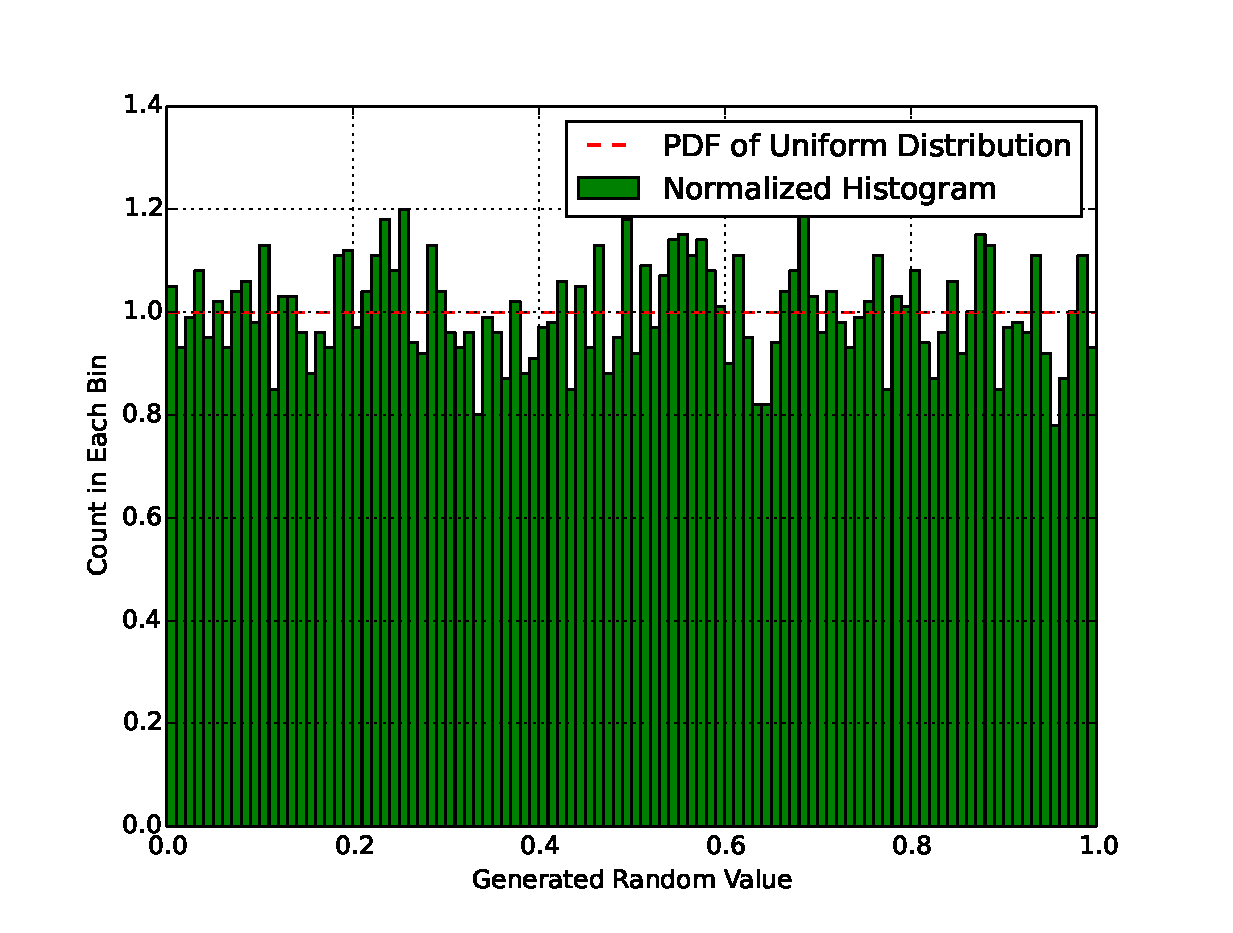
\includegraphics[scale=0.6]{rg_histogram.eps}
        \caption{Histogram of Uniform Random Values Generated by Numpy}
        \label{fig:uniform}
\end{figure}
\begin{figure}
        \centering
        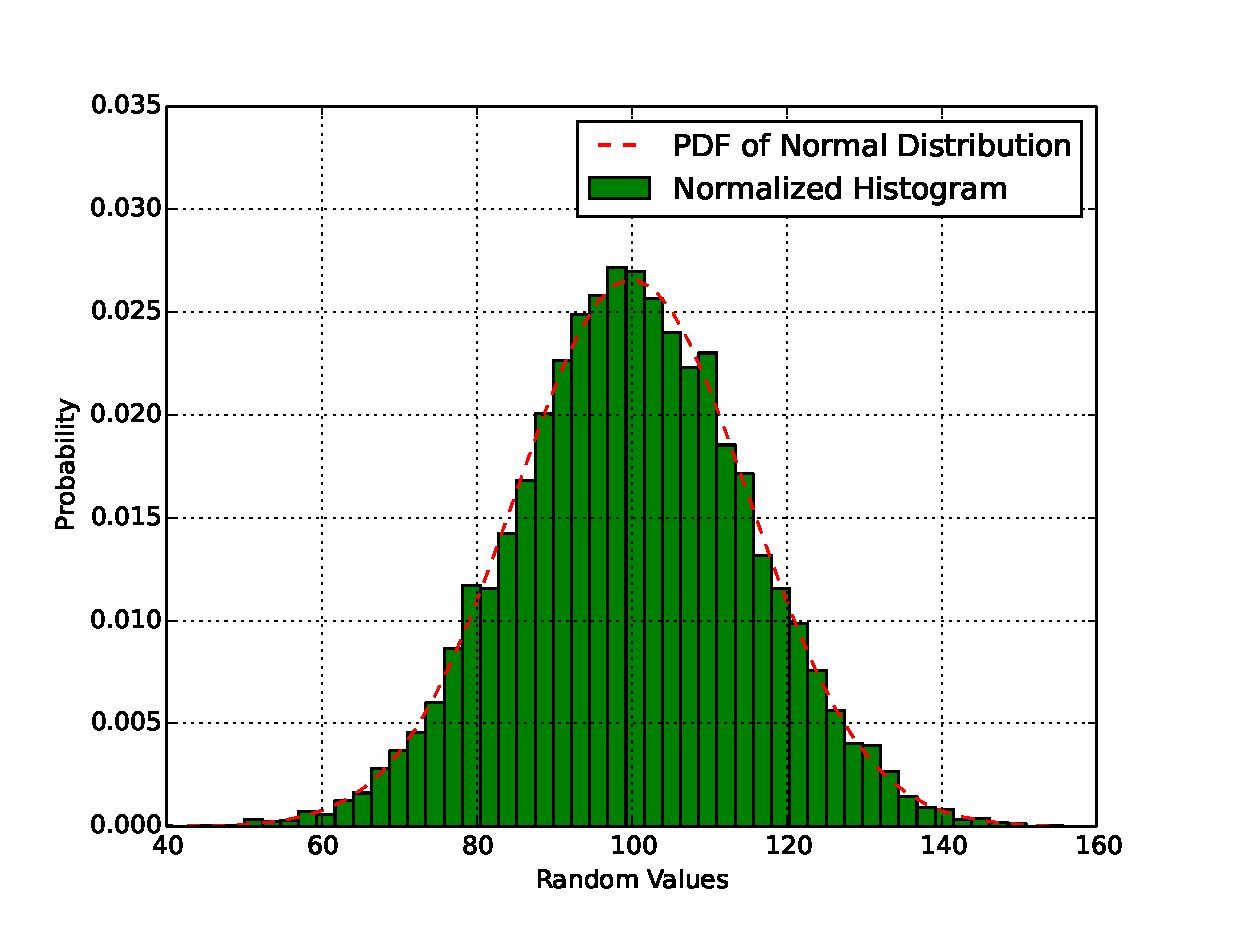
\includegraphics[scale=0.6]{rg_fitness.eps}
        \caption{Comparison to Best Fit Curve for Normal Distribution}
        \label{fig:normal}
\end{figure}

To generate different random value sequences, we feed the random generator a seed, which is the integral value of system current time.
That is the number of seconds since \textbf{Unix Epoch}.
We generated two sequences of 1000000 numbers each and use \textbf{t-test} to test statistically are they significantly different from each other.


\section{Eliminate Warm-up Period}
Using Algorithm \ref{alg:simulator} as core, we run \textbf{5000 simulations} for system A and system B under different initial states respectively.
For each simulation run, we \textbf{inject 1000 packets} into the system; the simulation terminates when these 1000 packets are all handled.
We choose to observe number of packets in the system during simulation.
Every time this system variable changes, we record its value and the happenning time moment.
After simulation, we process this log as follows.
First we create a observation time sequence with interval 1 magnitude less than arrival rate and ends at the finishing moment of the last departure event.
This ensure that we will not lost any accuracy.
For example, for system B where $\lambda=10$, the observation interval is 0.01.
Then based on the simulation log, we calculate the value of number of packet at every observation time point.
In this way we get the output for one simulation run.

We process all 5000 simulation logs and then can obtain 5000 simulation outputs.
Since simulation ends at different time, we only keep $m$ observations where $m = MIN$(length of all outputs).
Based on Welch graphical procedure, we average 5000 simulation outputs, observation by observation.
There are totally 4 cases to investigate: system A with 0 initial packets, system A with 7 initial packets, system B with 0 initial packets, system B with 4 initial packets.
All systems' Welch processing results are plotted in Figure \ref{fig:systemA:init0:all}, Figure \ref{fig:systemA:init7:all}, Figure \ref{fig:systemB:init0:all} and Figure \ref{fig:systemB:init4:all} respectively.
Since the nonstationary states only take up a very smal fraction of the entire output, we further zoom out the them in Figure \ref{fig:systemA:init0:warmup}, Figure \ref{fig:systemA:init7:warmup}, Figure \ref{fig:systemB:init0:warmup} and Figure \ref{fig:systemB:init4:warmup}.

\begin{figure*}
\centering
\subfloat[\textbf{System A with 0 Initial Packets}]{
        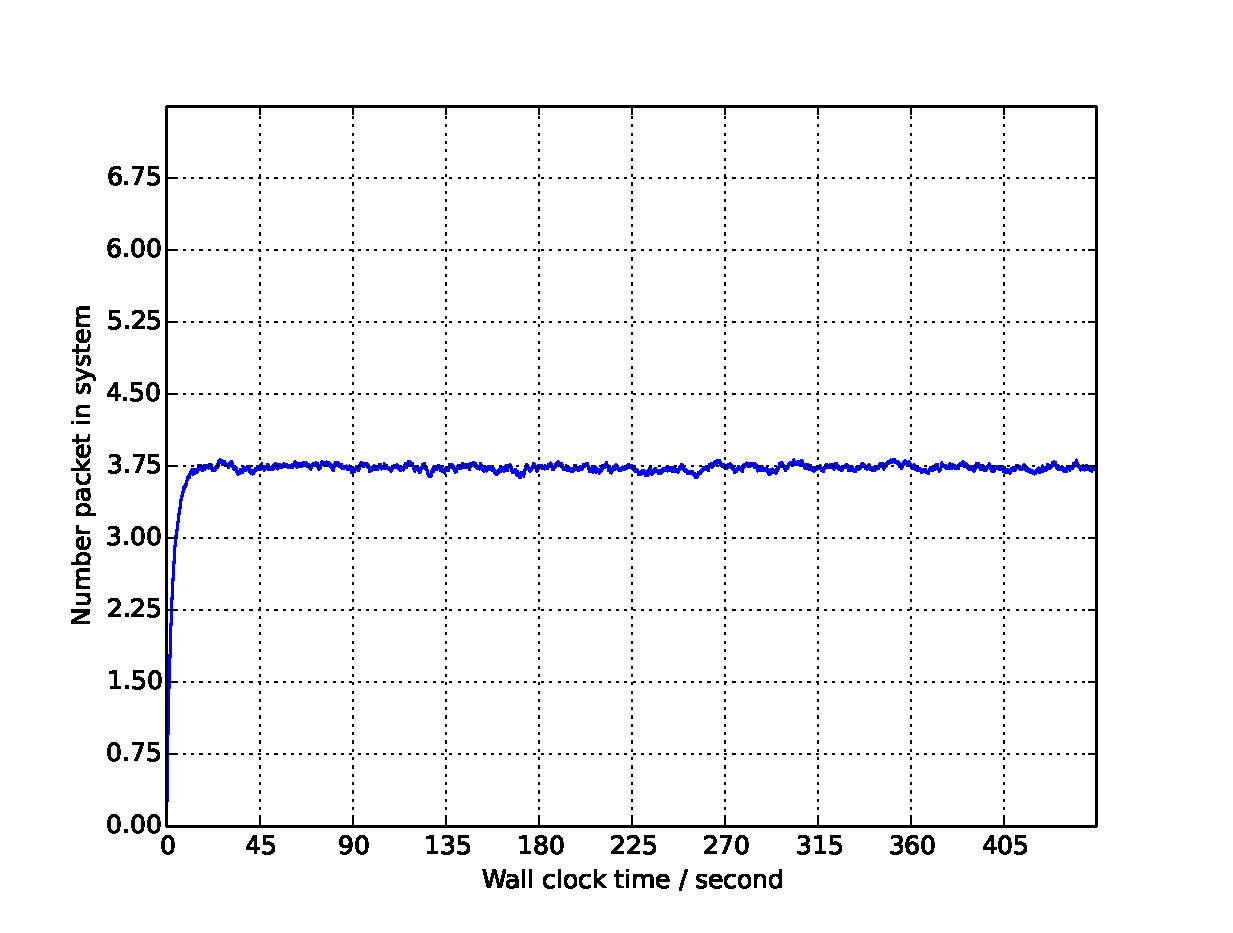
\includegraphics[scale=0.4]{Lmda2Init0Avg5000.eps}
        \label{fig:systemA:init0:all}
}
\hfill
\subfloat[\textbf{System A  with 7 Initial Packets}]{
        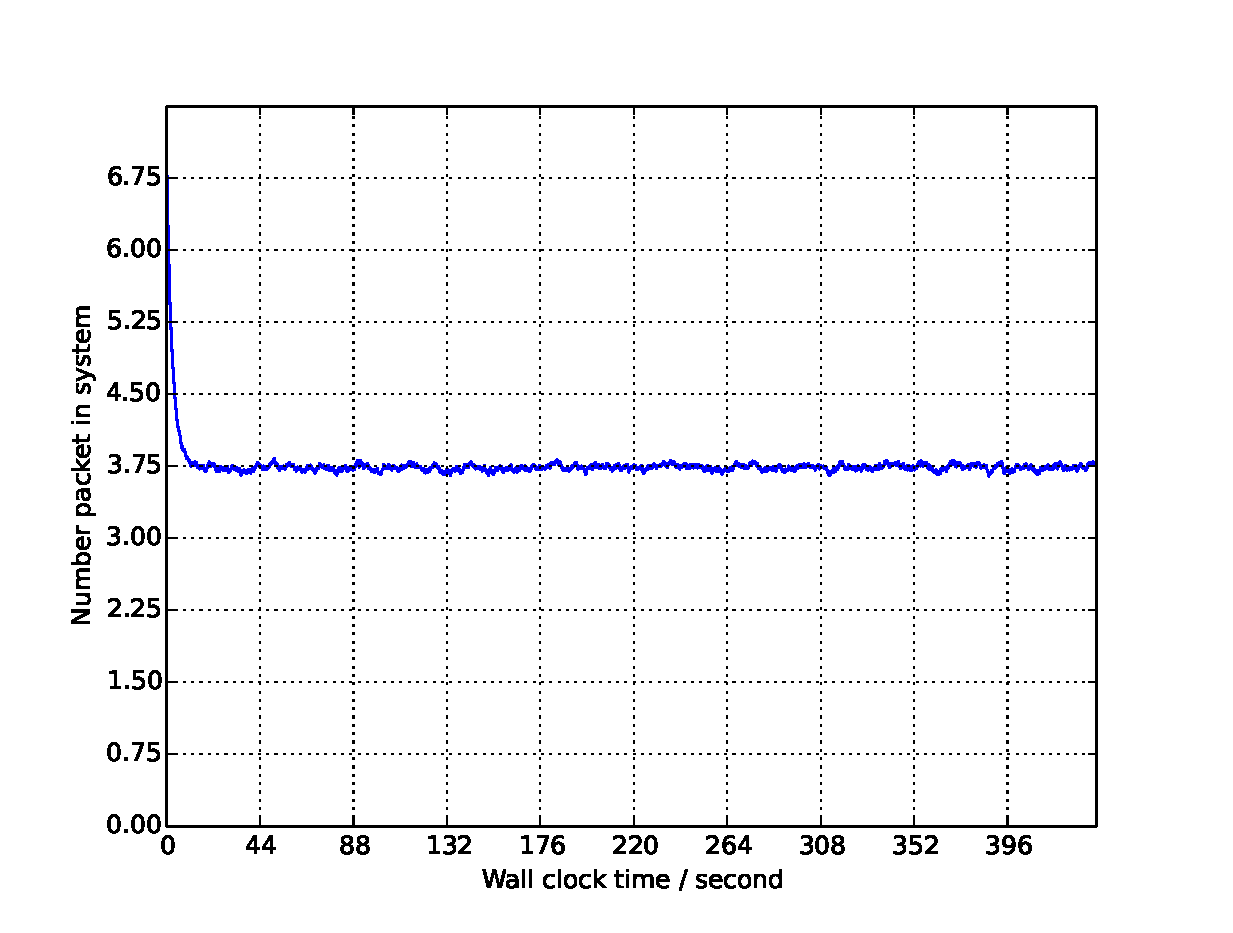
\includegraphics[scale=0.4]{Lmda2Init7Avg5000.eps}
        \label{fig:systemA:init7:all}
}
\\
\subfloat[\textbf{System B with 0 Initial Packets}]
{
        \includegraphics[scale=0.4]{Lmda10Init0Avg5000.eps}
        \label{fig:systemB:init0:all}
}
\hfill
\subfloat[\textbf{System B with 4 Initial Packets}]
{
        \includegraphics[scale=0.4]{Lmda10Init4Avg5000.eps}
        \label{fig:systemB:init4:all}
}
\caption{\textbf{Average 5000 Simulation Runs}}
\end{figure*}

As we can see from both the figures for entire simulation output and the figures for only nonstationary output, system A as well as system B will enter their respective stable state \textbf{regardless of the inital state}.
For system A, no matter we started from full buffer or empty buffer with empty server, the number of packet in the stable state is around \textbf{3.75}.
For system B, the number of packet in system will increase from different initial states and end up with close to a value of \textbf{6.75}.

\begin{figure*}
\centering
\subfloat[\textbf{System A with 0 Initial Packets}]{
        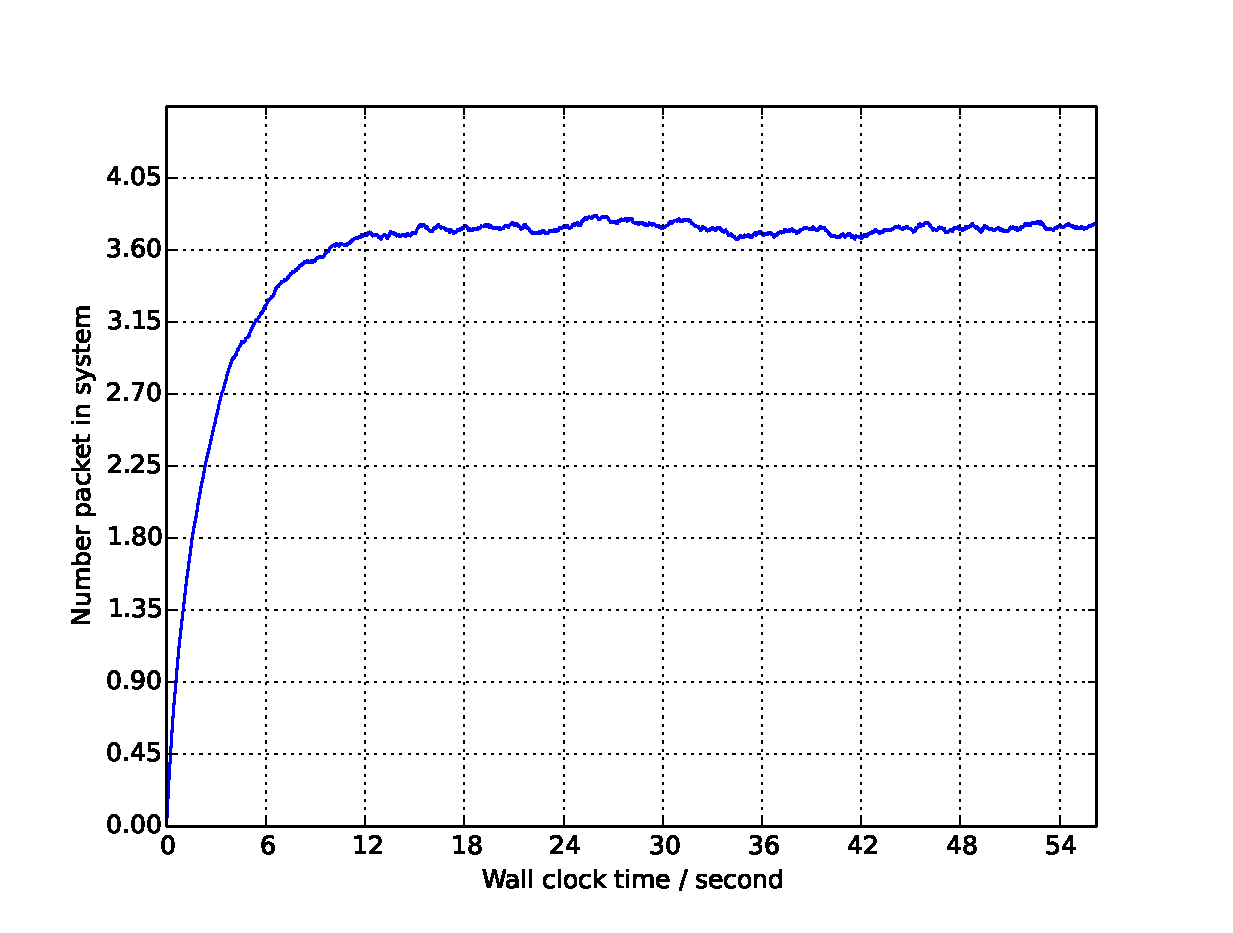
\includegraphics[scale=0.4]{Lmda2Init0OflAvg5000.eps}
        \label{fig:systemA:init0:warmup}
}
\hfill
\subfloat[\textbf{System A  with 7 Initial Packets}]{
        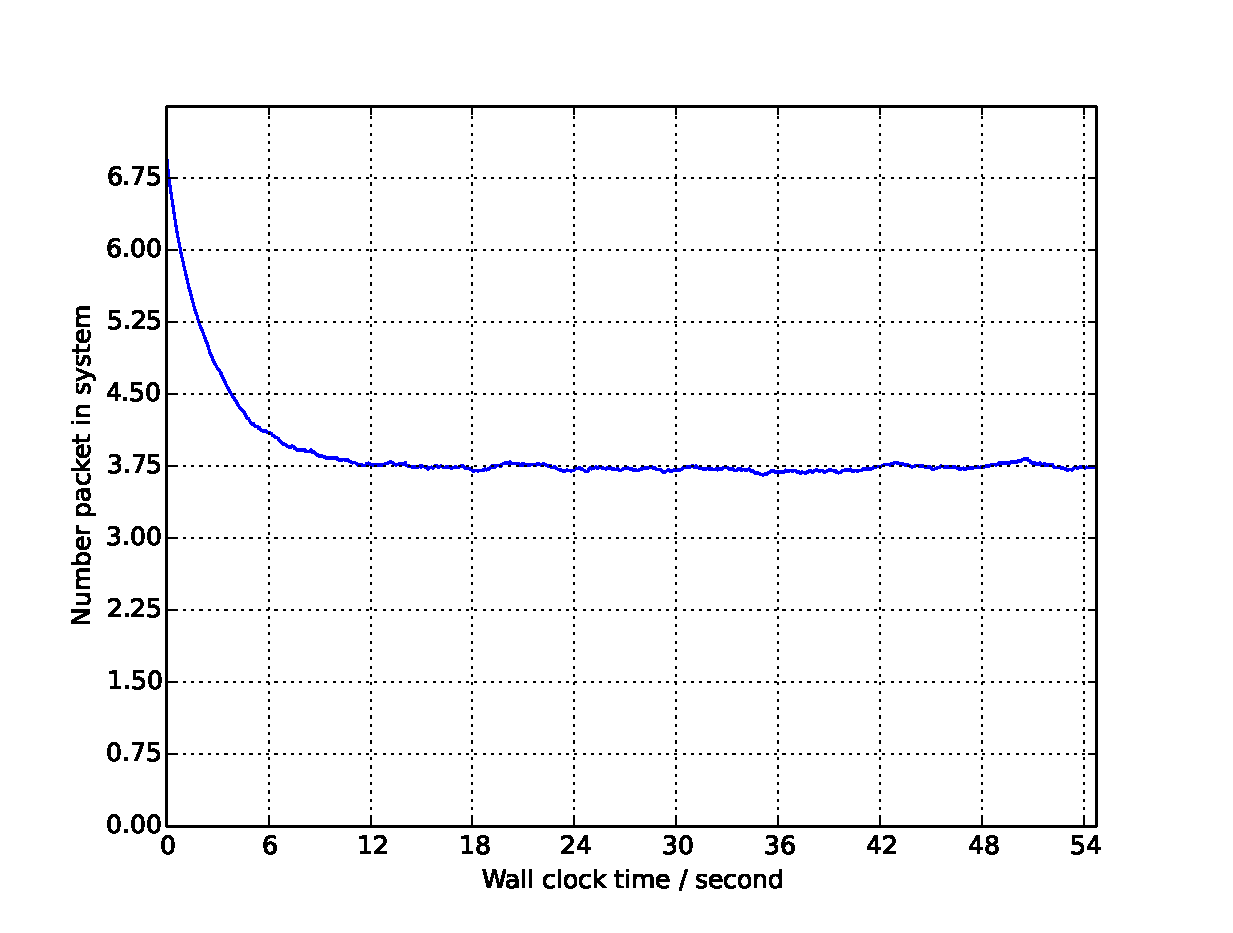
\includegraphics[scale=0.4]{Lmda2Init7OflAvg5000.eps}
        \label{fig:systemA:init7:warmup}
}
\\
\subfloat[\textbf{System B with 0 Initial Packets}]
{
        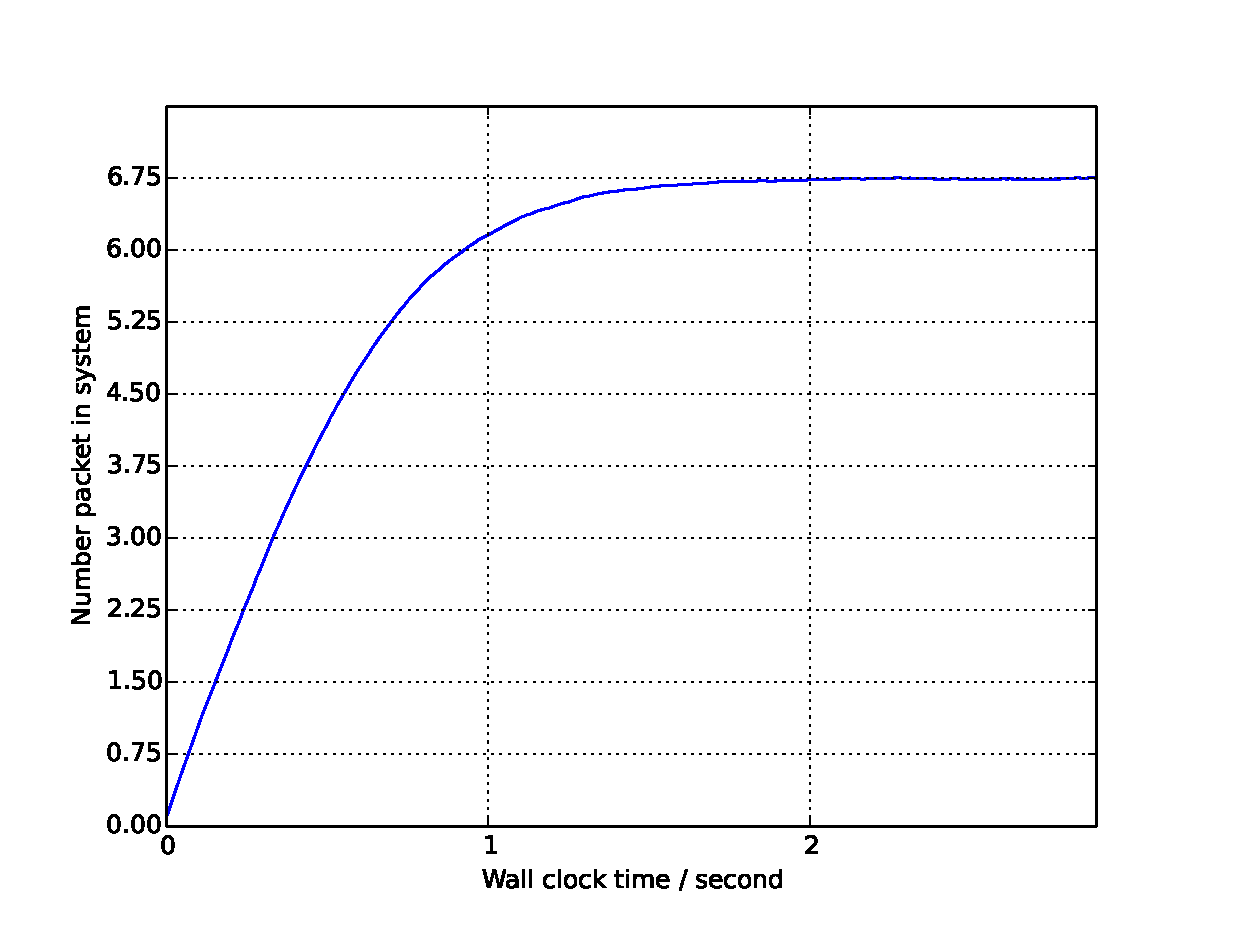
\includegraphics[scale=0.4]{Lmda10Init0OflAvg5000.eps}
        \label{fig:systemB:init0:warmup}
}
\hfill
\subfloat[\textbf{System B with 4 Initial Packets}]
{
        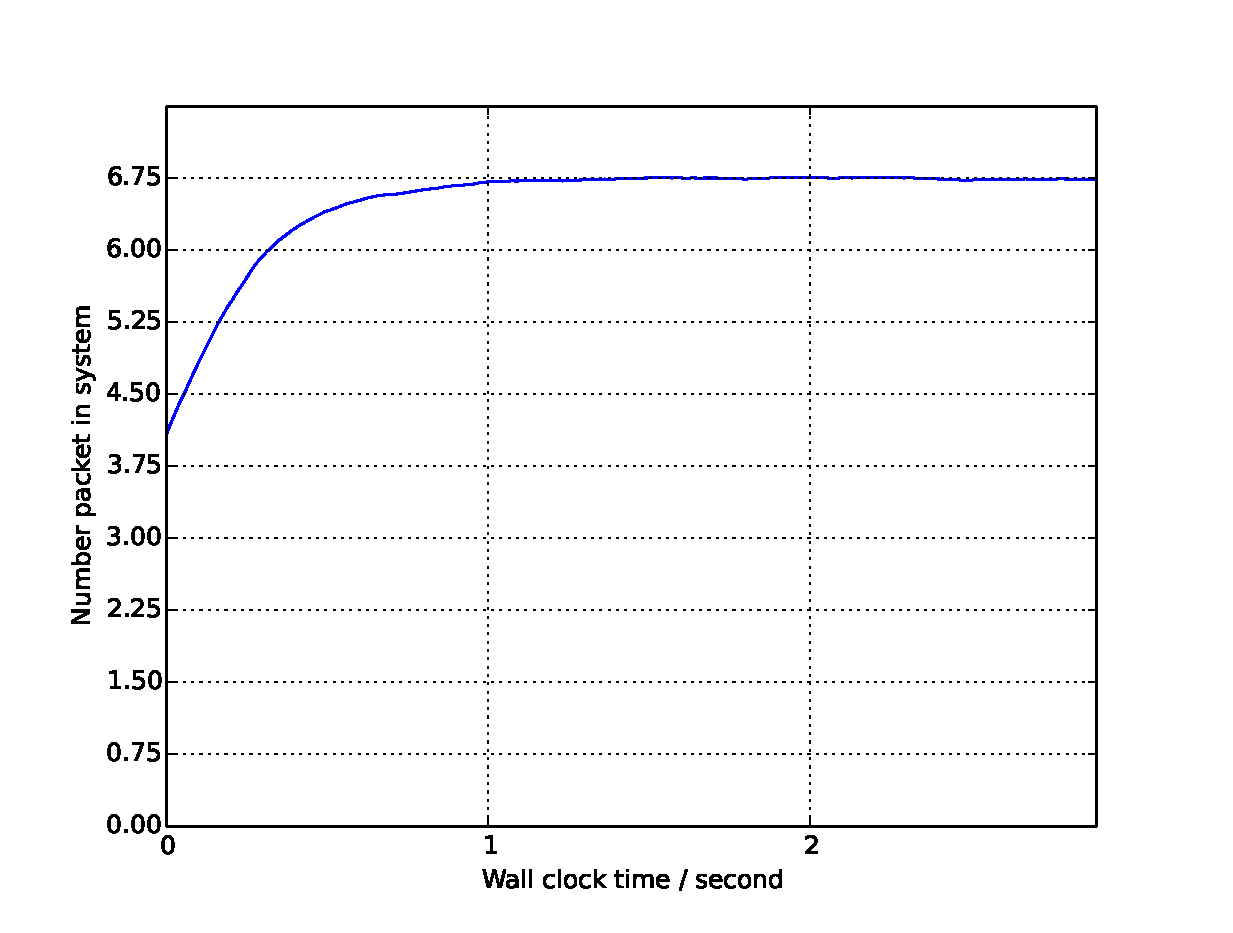
\includegraphics[scale=0.4]{Lmda10Init4OflAvg5000.eps}
        \label{fig:systemB:init4:warmup}
}
\caption{\textbf{Zoom out Nonstationary States}}
\end{figure*}


\section{System Properties at Stationary State}
In the last section, we have applied Welch graphical procedure and show the average simulation results of 5000 runs for each system with different initial state.
These figures clearly identifies the nonstationary and stationary states.
For system A, the time threshold for stable state is around 45 second in real time.
For system B, the time threshold for stable state is somewhere before 10 second.
However, we can pick a much larger time threshold when analysis system properies at the stationary state.
In the following statistic analysis, we treat the \textbf{first half} of the outputs as warmup peroid and just ignore them when calculating system properties.

For every simulation run, we first eliminate the data outputs belonging to warmup peroid, then we can calculate:
\begin{itemize}
\item \textbf{Blocking Probability} $P_B$ for a particular simulation run is defined by the ratio of number of dropped packets to the number of arrived packets:
\begin{align}
        \label{equ:block:prob}
        P_B = \frac{\textit{number of packets dropped}}{\textit{number of packets arrived}}
\end{align}

\item \textbf{Mean Spending Time} $S$, assuming there are totally $n$ served packet over time, is computed by:
\begin{align}
        \label{equ:mean:spending:time}
        S_s = \frac{\sum_{i=1}^{n}S_i}{n}
\end{align}
Here $S_i$ is the duration that packet $i$ spent in the system. 
As shown in Algorithm \ref{alg:simulator}, each accepted packet's spending time is recorded. 
Note that dropped packets are not counted in Equation \ref{equ:mean:spending:time}
\item \textbf{Mean Number of Packets} $E(N)$ of one run is calculated by:
\begin{align}
        \label{equ:mean:num:pkt}
        N_s = \sum_{i=0}^{7}\frac{i \times T_i}{T}
\end{align}
In Equation \ref{equ:mean:num:pkt}, $T_i$ is defined as the summation of durations that there are $i$ packets in the system.
$i$ can only range from 0 to 7, the capacity of our system.
To get $T_i$, we need log more information in simulation: the moment $t_i$ that the number of packets in system changes to $i$.
When simulation finishes, we can calculate the summation of durations that there are $i$ packets in the system.
$T$ is the entire duration of the simulated scenario, or the summation of all durations $T_i$.
\end{itemize}

With $N=5000$ independent simulations, we can further get the confidence interval for these calculated system properties.
The general formation of confidence interval for 90\% confidence level is
\begin{align}
        \label{equ:confidence:interval}
        \bar{X}\pm z_{1-\frac{\alpha}{2}}\sqrt{\frac{S^2}{N}}
\end{align}
where $z_{1-\frac{\alpha}{2}} = z_{0.95} = 1.645$ because $\alpha=0.1$.

To use Equation \ref{equ:confidence:interval}, for example,
to find the confidence level of mean number of packets in the system, we first need the estimator of the mean of $N_s$, which we treat as a random variable with unknown distribution:
\begin{align}
        \label{equ:estimate:mean:Ns}
        \overline{E(N_s)} = \frac{1}{N}\sum_{1}^{N}N_s[i]
\end{align}
where $N_s[i]$ is the mean number of packets in system for the $i^{th}$ simulation run and $N=5000$.
Then we need the estimator of the variance of $N_s$:
\begin{align}
        \label{equ:estimate:var:Ns}
        \overline{Var(N_s)} = \frac{\sum_{1}^{N}(N_s[i]-\overline{E(N_s)})^2}{N-1}
\end{align}
Based on Equation \ref{equ:confidence:interval}, we have the confidence interval for the mean number of packets in the system:
\begin{align}
        \label{equ:confidence:interval:Ns}
        \overline{E(N_s)} \pm \sqrt{\frac{Var(N_s)}{N}}
\end{align}

Table \ref{tab:confidence:interval} summarizes the confidence intervals for blocking probability, mean time spending in the system and mean number of packets in the system regarding to both system A and B with different initial state.
\begin{table}
%\centering
\caption{\textbf{Confidence Interval for $P_B,S_s$ and $N_s$}}
\begin{tabular}[b]{ccccc}
\hline
 & A with $x_{t=0}=0$ & A with $x_{t=0}=7$ & B with $x_{t=0}=0$ & B with $x_{t=0}=4$ \\
\hline
\hline
$P_b$ & 0.13264$\pm$0.00066 & 0.13318$\pm$0.00067 & 0.79902$\pm$0.00045 & 0.79958$\pm$0.00044 \\
\hline
$S_s$ & 2.15510$\pm$0.00816 & 2.15168$\pm$0.00827 & 3.35867$\pm$0.01221 & 3.37481$\pm$0.01219 \\
\hline
$N_s$ & 3.73037$\pm$0.01285 & 3.73350$\pm$0.01309 & 6.73854$\pm$0.00211 & 6.74043$\pm$0.00204 \\
\hline
\end{tabular}
\label{tab:confidence:interval}
\end{table}


%\begin{figure}[h]
%\centering
        %\includegraphics[width=0.8\textwidth, height=0.8\textheight]{progress.ps}
%\caption{Discovery Percentage as Function of Iteration for $R_1$ and $R_6$}
%\label{fig:progress}
%\end{figure}


%%%%%%%%%%%%%%%%%%%%%%%%%%%%%%%%%%%%%%%%%
%
%     Bibliography
%
%     Use an easy-to-remember tag for each entry - eg \bibitem{How97} for an article/book by Howie in 1997
%     To cite this publication in your text, write \cite{How97}.  To include more details such as
%     page, Chapter, Theorem numbers, use the form \cite[Theorem 6.3, page 42]{How97}.
%
%\begin{thebibliography}{99}

% 
% The usual convention for mathematical bibliographies is to list alphabetically
% by first-named author (then second, third  etc. author then date)
% websites with no author names should go by the site name
%


% Typical layout for reference to a journal article
%
%\bibitem{Bovey}
%J. D. Bovey, M. M. Dodson,                         % author(s)
%The Hausdorff dimension of systems of linear forms % article name
%{\em Acta Arithmetica}                             % journal name - italics
%{\bf 45}                                           % volume number - bold
%(1986), 337--358.                                   % (year), page range

%% Typical layout for reference to a book
%%
%\bibitem{Cassels}
%J. W. S. Cassels,                                  % author(s)
%{\em An Introduction to Diophantine Approximation},% title - italics
%Cambridge University Press, Cambridge, 1965.       % Publisher, place, date.

%% Typical layout for reference to a website
%%
%\bibitem{GAP}
%The GAP Group, GAP -- Groups, Algorithms, and Programming,  % Site name
%Version 4.5.6; 2012. % other information
%(http://www.gap-system.org)  % URL


%% Typical layout for reference to an online article
%%
%\bibitem{Howie}
%J. Howie,                                            % author(s)
%{\em Generalised triangle groups of type $(3,5,2)$}, % article name - italics
%http://arxiv.org/abs/1102.2073                       % URL
%(2011).                                              % (year)
%\end{thebibliography}

\end{document}
